\chapter{Multithreading}

\begin{summary}
Multithreading is a crucial concept in Java. It allows two or more parts of a program to be executed simultaneously to maximize CPU utilization. Video games, computer simulations, web servers, and browsers are examples of applications where the use of multithreading is essential. Various Java frameworks rely on multithreading. Therefore, it is important to understand the basic concepts.

Additionally, with the introduction of virtual threads as part of Project Loom, Java’s capability for handling concurrent operations is set to increase, allowing for a much larger number of threads to be managed with significantly less overhead. This is particularly beneficial for IO-bound and server-side applications.

Furthermore, mastering asynchronous programming techniques, such as those offered by CompletableFuture and Spring's asynchronous methods, enables developers to write non-blocking code that can perform tasks in the background, improving application responsiveness and overall throughput.
\end{summary}

\section{Introduction to Multithreading}

To fully grasp the term multithreading, we begin by explaining the difference between a thread and a process. A process is a program that is being executed. It can consist of one or more execution paths. These mini-processes within a program are called threads. Multithreading refers to writing a program in which multiple threads are implemented that can be executed simultaneously.

The different threads within a process can be executed at the same time, allowing the CPU to be utilized to its maximum potential. In a single-core CPU, there is a scheduler that decides which thread is executed and manages context switching between the different threads. This context switching happens so quickly that it seems as though multiple things are happening at once in the program. For example, imagine playing Pac-Man on a single-core CPU. The ghosts continuously move across the screen while you simultaneously input keyboard commands to control Pac-Man and dodge the ghosts.

In a multi-core CPU, the execution of different threads can genuinely occur simultaneously. However, a scheduler is still necessary to ensure that all threads get an equal share of processing time.

\begin{figure}[H]
  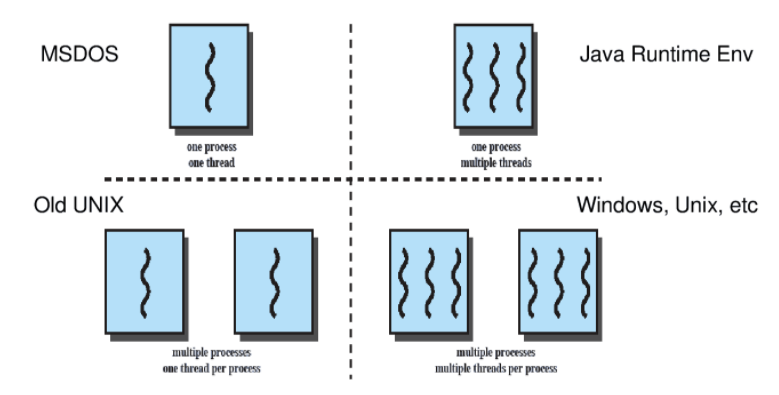
\includegraphics[width=\linewidth]{images/h9/process_threads.png} 
  \caption{Relatie tussen proces en threads}
  \label{fig:proces_thread}
\end{figure}

\begin{figure}[H]
  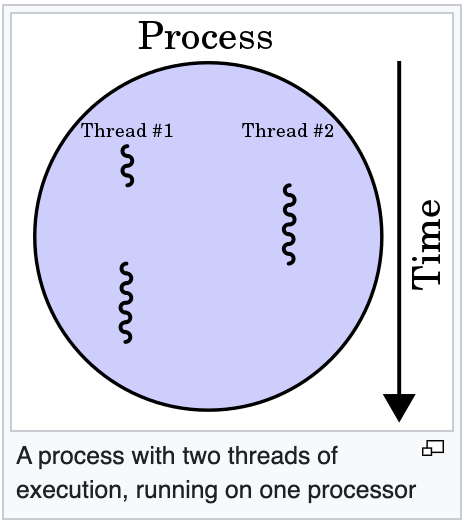
\includegraphics[scale=1]{images/h9/process_with_two_threads.png}
  \label{fig:proces_thread_2}
\end{figure}

Multitasking is the ability to perform more than one task at the same time. Java therefore provides thread-based multitasking. Within a process, threads share a portion of memory. This portion, known as the heap, is where the objects reside. Each thread also has a piece of private memory used during the execution of the thread, referred to as the stack. When the scheduler decides to activate another thread within a process, this context switch is carried out very efficiently.

\section{Use cases for multithreading}

Web Servers: In web servers, threads can handle multiple client requests simultaneously, improving the server's ability to serve more clients efficiently without waiting for each request to be processed sequentially.
Multimedia Applications: Applications that deal with multimedia processing, like video players or audio streaming services, use threads to ensure smooth playback while simultaneously downloading or buffering future content.
Financial Applications: In finance, real-time transaction processing systems use threads to handle high volumes of concurrent transactions, ensuring data consistency and quick response times during market hours.
Gaming: Modern video games use multithreading to separate logic and rendering processes, and to manage real-time user inputs along with game state management without lag.
Scientific Computing: Applications that perform complex simulations and data analysis can use threads to distribute the computational load across multiple CPU cores, significantly speeding up processing times.
Mobile Applications: Mobile apps often use threads to perform background tasks such as data synchronization, fetching updates, or performing lengthy computations while keeping the user interface responsive.

\section{Basics of Threads}

Threads are objects in Java. All Java programs have at least one thread, the main thread, which is created by the JVM (Java Virtual Machine) when the program is started. The main() method is executed by the main thread. In addition, you can create additional threads. You create these objects by either making a subclass of the Thread class or by implementing the functional interface Runnable. We will look at both possibilities.


\subsection{Creating Threads Using the Thread Class}

When you create a subclass of the Thread class, you override the run() method. The run() method contains the instructions that the thread will execute once you call the start() method.

\begin{lstlisting}
public class WorkerThread extends Thread {

	@Override
	public void run() {
		System.out.println("Line A (" + Thread.currentThread().getName() + ")");
		System.out.println("Line B (" + Thread.currentThread().getName() + ")");
		System.out.println("Line C (" + Thread.currentThread().getName() + ")");
		System.out.println("Line D (" + Thread.currentThread().getName() + ")");
		System.out.println("Line E (" + Thread.currentThread().getName() + ")");
	}

	public static void main(String[] args) {
		WorkerThread workerThread = new WorkerThread();
		workerThread.start();
		System.out.println("Line 1 (" + Thread.currentThread().getName() + ")");
		System.out.println("Line 2 (" + Thread.currentThread().getName() + ")");
		System.out.println("Line 3 (" + Thread.currentThread().getName() + ")");
	}
}
\end{lstlisting}


Once an instance of the WorkerThread class has been started, the scheduler alternates between the main thread and the WorkerThread instance. On a single-processor computer, it appears as though the threads are being executed simultaneously, while on a multi-processor computer, the threads can actually be executed at the same time.

Here is a possible sequence of the program:

\begin{verbatim}
Line A (Thread-0)
Line 1 (main)
Line B (Thread-0)
Line 2 (main)
Line C (Thread-0)
Line 3 (main)
Line D (Thread-0)
Line E (Thread-0)
\end{verbatim}


\subsection{Implementing the Runnable Interface}

A second way to program a thread is by creating a class that implements the java.lang.Runnable interface. Here as well, you must provide an implementation of the run() method. To start the thread, you need to pass an instance of the class that implements the Runnable interface as a parameter to a constructor of the Thread class. Then, you can call the start() method.

\begin{lstlisting}
public class WorkerThread2 implements Runnable {

	@Override
	public void run() {
		System.out.println("Line A (" + Thread.currentThread().getName() + ")");
		System.out.println("Line B (" + Thread.currentThread().getName() + ")");
		System.out.println("Line C (" + Thread.currentThread().getName() + ")");
		System.out.println("Line D (" + Thread.currentThread().getName() + ")");
		System.out.println("Line E (" + Thread.currentThread().getName() + ")");
	}

	public static void main(String[] args) {
		WorkerThread2 workerThread = new WorkerThread2();
		new Thread(workerThread).start();
		System.out.println("Line 1 (" + Thread.currentThread().getName() + ")");
		System.out.println("Line 2 (" + Thread.currentThread().getName() + ")");
		System.out.println("Line 3 (" + Thread.currentThread().getName() + ")");
	}
}
\end{lstlisting}

A common mistake is calling the run() method instead of the start() method. At first glance, this may not seem problematic. However, it does NOT result in a multithreaded program. Instead, the main thread will execute the instructions of the run() method. Test this out by calling run() instead of start() in the program above. Make sure you avoid this mistake!

\subsection{Runnable as a Lambda Expression}

Since the Runnable interface is a functional interface, you can also use a lambda expression to simplify your code. This approach is particularly useful for creating quick runnables without having to create a whole new class. Lambda expressions provide a concise way to implement the single abstract method of a functional interface.

Here is a simple example of using a lambda expression to implement Runnable:

\begin{lstlisting}
public class WorkerThread3 {

	public static void main(String[] args) {
		new Thread(() -> {
			System.out.println("Line A (" + Thread.currentThread().getName() + ")");
			System.out.println("Line B (" + Thread.currentThread().getName() + ")");
			System.out.println("Line C (" + Thread.currentThread().getName() + ")");
			System.out.println("Line D (" + Thread.currentThread().getName() + ")");
			System.out.println("Line E (" + Thread.currentThread().getName() + ")");
		}).start();
		System.out.println("Line 1 (" + Thread.currentThread().getName() + ")");
		System.out.println("Line 2 (" + Thread.currentThread().getName() + ")");
		System.out.println("Line 3 (" + Thread.currentThread().getName() + ")");
	}
}
\end{lstlisting}

In this example, the lambda expression () -> {...} implements the Runnable interface. It defines what the thread will do when executed, without the need for a separate Runnable class. This simplifies the code and makes it more readable, especially for short tasks or when working within a context where adding new classes would be cumbersome.


\subsection{Thread class versus Runnable Interface}

It may be a bit confusing that you have two possibilities for implementing threads. However, there are important differences between the two implementations. When you create a subclass of Thread, the objects of this class are 'real' thread objects and you, as a developer, have full control over the thread. When you use the Runnable interface, you are essentially only defining the work that needs to be performed by the thread. You then have no control over the thread itself.

If you make a subclass of the Thread class, you cannot use a second superclass because Java does not allow multiple inheritance. Therefore, if you want to inherit from another superclass, you use the Runnable interface.

\subsection{Virtual threads}

Real threads, or platform threads, in Java correspond directly to native OS threads. Each Java thread is a thin wrapper around these OS-level threads, which means they are managed and scheduled by the operating system. Real threads are powerful because they can run truly concurrently on multicore processors, leveraging parallelism. However, they also come with higher costs in terms of context switching, memory usage, and scheduling overhead, which can become significant when managing a large number of threads.

Virtual threads, introduced as part of Project Loom, aim to address the scalability issues posed by real threads. Unlike real threads, virtual threads are lightweight, managed entirely by the Java Virtual Machine (JVM) rather than the operating system. They are designed to have a low memory footprint and allow for massive concurrency. Virtual threads achieve this by decoupling the thread lifecycle from the underlying OS thread, using a scheduling technique known as 'fibers', which are scheduled by the JVM onto a smaller number of real threads.

\begin{lstlisting}
public class WorkerThread4 {

	public static void main(String[] args) {
		Thread virtualThread = Thread.startVirtualThread(() -> {
			System.out.println("Line A (" + Thread.currentThread().getName() + ")");
			System.out.println("Line B (" + Thread.currentThread().getName() + ")");
			System.out.println("Line C (" + Thread.currentThread().getName() + ")");
			System.out.println("Line D (" + Thread.currentThread().getName() + ")");
			System.out.println("Line E (" + Thread.currentThread().getName() + ")");
		});
		System.out.println("Line 1 (" + Thread.currentThread().getName() + ")");
		System.out.println("Line 2 (" + Thread.currentThread().getName() + ")");
		System.out.println("Line 3 (" + Thread.currentThread().getName() + ")");

        try {
            virtualThread.join(); // wait for the virtual thread to end
        } catch (InterruptedException e) {
            throw new RuntimeException(e);
        }
    }
}
\end{lstlisting}


\begin{lstlisting}
import java.util.concurrent.ExecutorService;
import java.util.concurrent.Executors;
import java.util.concurrent.ThreadFactory;
import java.util.concurrent.TimeUnit;

public class ThreadFactoryWithVirtualThread {

    public static void main(String[] args) {
        ThreadFactory virtualThreadFactory = Thread.ofVirtual().name("MyVirtualThread-", 0).factory();

        ExecutorService executor =
                Executors.newFixedThreadPool(4, virtualThreadFactory);

        for (int i = 0; i < 8; i++) {
            executor.submit(() -> {
                System.out.println("Running task in a virtual thread: "
                        + Thread.currentThread().getName());
            });
        }

        shutdownAndAwaitTermination(executor);
    }

    private static void shutdownAndAwaitTermination(ExecutorService executorService) {
        executorService.shutdown(); // Disable new tasks from being submitted
        try {
            // Wait a while for existing tasks to terminate
            if (!executorService.awaitTermination(10, TimeUnit.SECONDS)) {
                executorService.shutdownNow(); // Cancel currently executing tasks
                // Wait a while for tasks to respond to being cancelled
                if (!executorService.awaitTermination(10, TimeUnit.SECONDS)) {
                    System.err.println("Executor service failed to terminate.");
                }
            }
        } catch (InterruptedException ex) {
            executorService.shutdownNow();       // (Re-)Cancel if current thread also interrupted
            Thread.currentThread().interrupt();           // Preserve interrupt status
        }
    }
}
\end{lstlisting}

Here, we demonstrate the use of a ThreadFactory with virtual threads. We create a virtual thread factory using Thread.ofVirtual().factory(), and then use it to create a fixed-size thread pool with Executors.newFixedThreadPool(). Tasks submitted to this pool execute in virtual threads created by the virtual thread factory.

\begin{verbatim}
Running task in a virtual thread: MyVirtualThread-2
Running task in a virtual thread: MyVirtualThread-1
Running task in a virtual thread: MyVirtualThread-0
Running task in a virtual thread: MyVirtualThread-3
Running task in a virtual thread: MyVirtualThread-2
Running task in a virtual thread: MyVirtualThread-1
Running task in a virtual thread: MyVirtualThread-0
Running task in a virtual thread: MyVirtualThread-3
\end{verbatim}

\section{Thread life cycle}

A Java thread always has one of the following statuses:
\begin{itemize}
\item NEW\\
As soon as you create a Thread object, it has the status \textit{NEW}. As soon as the \textit{start()} method is called, the status of the thread changes from NEW to RUNNABLE.
\item RUNNABLE\\
A thread that is executed in the JVM (Java Virtual Machine) is in this status. There are 2 possibilities: either the thread is effectively being executed, or the thread is ready to be executed but is waiting for an available processor.
\item BLOCKED\\
A thread is in the BLOCKED status when the thread must wait to execute a synchronized code fragment. A synchronized code fragment is a method or part of a method that can only be executed by one thread at a time. If one thread is executing this code, other threads that want to start with this code fragment must wait. We will delve deeper into synchronization in this section.
\item WAITING\\
A thread is in the WAITING status if it is waiting for another thread that needs to perform a certain action first.
\item TIMED\_WAITING\\
A thread is in the status timed\_waiting just like in the waiting status if it is waiting for another thread to perform a certain action. The difference, however, is that the thread has a timeout set and will proceed after the preset time.
\item TERMINATED\\
A thread that has completed its task is in the status TERMINATED.
\end{itemize}

\begin{figure}[H]
  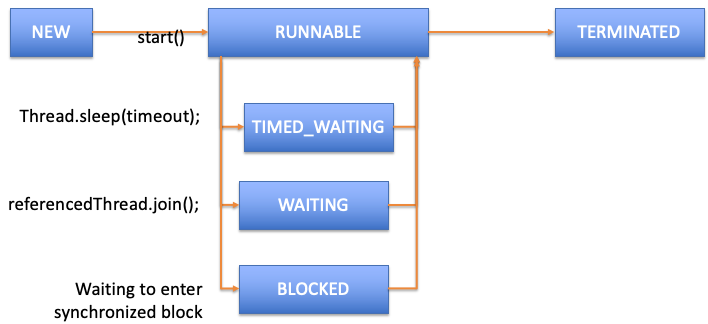
\includegraphics[width=\linewidth]{images/h9/thread_life_cycle.png}
  \label{fig:thread_life_cycle}
\end{figure}

\section{Common thread methods}


\subsection{Thread.sleep()}

The Thread.sleep() method can be used to pause a thread for a specified amount of time (expressed in milliseconds).
Note that this method is a static method.
When the Thread.sleep() instruction is executed, the thread scheduler will place the caller in WAIT status for the specified time. Once this time has passed, the thread's status becomes RUNNABLE again, and then it will have to wait until the CPU is available to continue execution. The actual time that the thread will thus 'sleep' is therefore dependent on the thread scheduler.

\begin{lstlisting}
public class WorkerThreadWithSleep extends Thread {

	@Override
	public void run() {
		System.out.println("Line A (" + Thread.currentThread().getName() + ")");
		try {
			Thread.sleep(5000);
		} catch (InterruptedException e) {
			e.printStackTrace();
		}
		System.out.println("Line B (" + Thread.currentThread().getName() + ")");
		System.out.println("Line C (" + Thread.currentThread().getName() + ")");
		System.out.println("Line D (" + Thread.currentThread().getName() + ")");
		System.out.println("Line E (" + Thread.currentThread().getName() + ")");
	}

	public static void main(String[] args) {
		WorkerThreadWithSleep workerThread = new WorkerThreadWithSleep();
		System.out.println(workerThread.getState());
		workerThread.start();
		System.out.println(workerThread.getState());
		System.out.println("Line 1 (" + Thread.currentThread().getName() + ")");
		System.out.println("Line 2 (" + Thread.currentThread().getName() + ")");
		System.out.println("Line 3 (" + Thread.currentThread().getName() + ")");
		System.out.println(workerThread.getState());
	}
}
\end{lstlisting}

After printing 'Line A...', the workThread goes to sleep for 5 seconds. The status of the workerThread then becomes TIMED_WAITING, and the main thread can continue its activities. When the 5 seconds are up, the workThread can resume work.

\begin{oefening}
Create a class \textbf{Talker} that is a subclass of the class \textbf{java.util.Thread}.
You should include a property \textbf{id} (int) in this subclass and a constructor that allows you to create a Talker object and pass the id as a parameter.
When the thread is started, it will print its id 10 times, each time with a half-second pause.
Create 4 instances of the Talker class in the main program and start the threads.
\\
Then modify the Talker class so that it implements the Runnable interface. What changes do you need to make in your code?
\end{oefening}

\subsection{referencedThread.join()}

When a running thread calls the instruction referencedThread.join(), the executing thread enters the WAIT status. The thread remains waiting until the referencedThread is completely finished. If the referencedThread was already finished, the executing thread can simply continue with its tasks and does not need to wait, of course.


\begin{lstlisting}
public class WorkerThreadWithJoin extends Thread {

	@Override
	public void run() {
		System.out.println("Line A (" + Thread.currentThread().getName() + ")");
		System.out.println("Line B (" + Thread.currentThread().getName() + ")");
		System.out.println("Line C (" + Thread.currentThread().getName() + ")");
		System.out.println("Line D (" + Thread.currentThread().getName() + ")");
		System.out.println("Line E (" + Thread.currentThread().getName() + ")");
	}

	public static void main(String[] args) {
		WorkerThreadWithJoin workerThread = new WorkerThreadWithJoin();
		System.out.println(workerThread.getState());
		workerThread.start();
		System.out.println(workerThread.getState());
		System.out.println("Line 1 (" + Thread.currentThread().getName() + ")");
		try {
			workerThread.join();
		} catch (InterruptedException e) {
			e.printStackTrace();
		}
		System.out.println("Line 2 (" + Thread.currentThread().getName() + ")");
		System.out.println("Line 3 (" + Thread.currentThread().getName() + ")");
		System.out.println(workerThread.getState());
	}
}
\end{lstlisting}

After displaying 'Line 1...', the main thread will wait until the workerThread is completely finished. Only after the workerThread has concluded will the main thread resume execution. Therefore, the program will produce the following output.

\begin{verbatim}
NEW
RUNNABLE
Line 1 (main)
Line A (Thread-0)
Line B (Thread-0)
Line C (Thread-0)
Line D (Thread-0)
Line E (Thread-0)
Line 2 (main)
Line 3 (main)
TERMINATED
\end{verbatim}


\begin{oefening}
We are going to search for the integer between 1 and 10000 that has the greatest number of divisors. A divisor is a number that divides another without leaving a remainder. We want to know which number this is and how many divisors it has.

Create a class DivisorCounter. You can pass a minimum and maximum number to the constructor. This will be the range of numbers that the thread will test.
Initially, set these values to 1 and 10000. Write a method that can find the number with the highest number of divisors within this range. This method may be called directly from the constructor.
The found number (and the number of divisors) must be stored in a member variable.

Add a main() method that performs the calculation and prints the result.
The result should be either 7560 or 9240, as both numbers have 64 divisors.

Also, make sure you print the execution time of your calculation.

Try increasing the range to 50000 or 100000 numbers, and you will see that the execution time increases exponentially.

Modify your code so that you can divide the calculation into subproblems and have each part executed by a separate thread. Thus, you will make the DivisorCounter class a thread.
Then, in the main() method, write the necessary code to start several threads with a part of the range. Once the threads are done executing, finally make the necessary comparisons to determine which number has the greatest number of divisors from the entire range.

Check if your program now executes faster. With 10 threads, we get the following result:
\begin{verbatim}
Range [1-50000]
Getal: 45360
Aantal delers: 100
Tijd: 1.684 seconden
\end{verbatim}
\end{oefening}

\section{Thread synchronization}
Multithreading is a powerful technique, but it makes programs more difficult to control and debug, especially when threads start sharing resources.

In the following example, the shared resource is a cookie jar.
Here is the CookieBox class.

\begin{lstlisting}
public class CookieBox {

	private int numberOfCookies;

	public CookieBox(int numberOfCookies) {
		this.numberOfCookies = numberOfCookies;
	}

	public boolean takeCookie() {
			if (numberOfCookies > 0) {
				numberOfCookies--;
				return true;
			}
			return false;
	}
}
\end{lstlisting}

The class Child is a thread.

\begin{lstlisting}
public class Child extends Thread {

	private int numberOfCookies;
	private CookieBox cookieBox;
	private String name;

	public Child(String name, CookieBox cookieBox) {
		this.cookieBox = cookieBox;
		this.name = name;
	}

	@Override
	public void run() {
		while (cookieBox.takeCookie()) {
			numberOfCookies++;
			try {
				Thread.sleep(5);
			} catch (InterruptedException e) {
				e.printStackTrace();
			}
		}
		System.out.println(name + " had " + numberOfCookies + " cookies");
	}

	public int getNumberOfCookies() { return numberOfCookies; }
}
\end{lstlisting}

\begin{lstlisting}
public class EatingCookies {

	public static void main(String[] args) {
		CookieBox cookieBox = new CookieBox(50);
		Child[] children = { new Child("Bram", cookieBox),
				new Child("Sophie", cookieBox),
				new Child("Elke", cookieBox),
				new Child("Robin", cookieBox),
				new Child("Sammy", cookieBox),
				new Child("Max", cookieBox) };
        for (Child child : children) {
            child.start();
        }
        for (Child child : children) {
            try {
                child.join();
            } catch (InterruptedException e) {
                e.printStackTrace();
            }
        }
		System.out.println("Total amount of cookies: " +
				Arrays.stream(children)
						.mapToInt(Child::getNumberOfCookies)
						.sum());
	}
}
\end{lstlisting}

We create one CookieBox with 50 cookies and 6 Child threads that will all take cookies from this cookie jar. We start the 6 threads and pause the main() thread until all the Kind threads are finished and the cookie jar is empty. Then, we will ask the Kind threads how many cookies they have eaten.

\begin{verbatim}
Sammy had 10 cookies
Bram had 9 cookies
Sophie had 10 cookies
Elke had 9 cookies
Max had 10 cookies
Robin had 10 cookies
Total amount of cookies: 58
\end{verbatim}

Despite the fact that there are only 50 cookies in the cookie jar, the Child threads will still manage to eat a total of 58 cookies together. Clearly, something is going wrong.

\begin{figure}[H]
  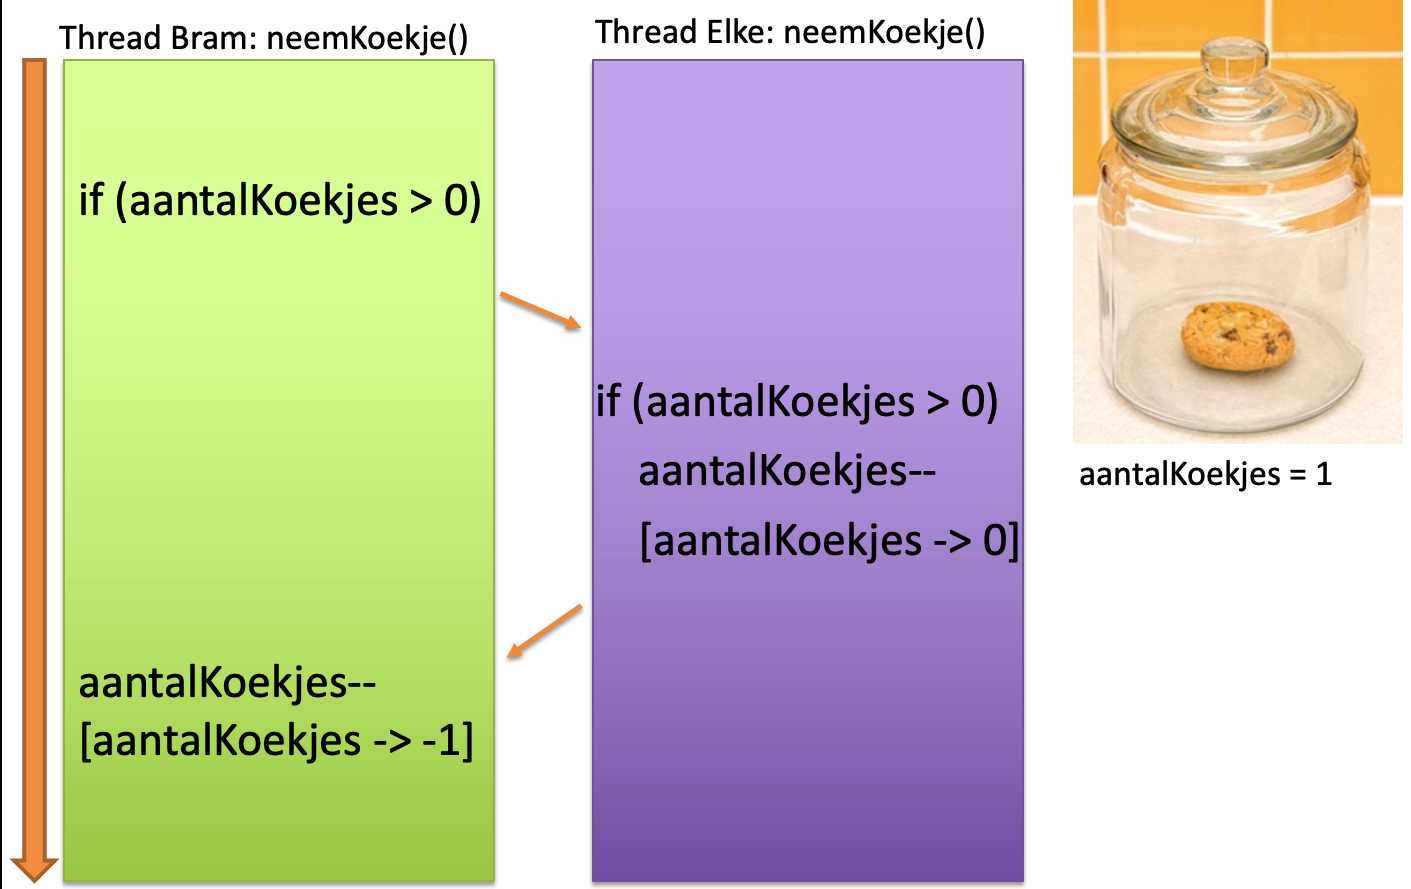
\includegraphics[width=\linewidth]{images/h9/koekjesdoos.png}
  \label{fig:concurrent_access}
\end{figure}

In the image above, we illustrate what goes wrong.
We assume that we have one processor and that there are two threads (Bram and Elke) executing the takeCookie() method simultaneously. There is still one cookie left in the cookie jar.
Thread Bram takes its turn and checks if there is a cookie available. This is the case, so the condition returns true. However, the thread scheduler decides it's Elke's turn. This thread checks if there is still a cookie and decreases the number of cookies by one. Now, it's Bram's turn again. The thread resumes its operations at the point of decreasing the number of cookies, and now we have -1 cookies.

The error occurred because thread Bram, after checking if there was still a cookie, did not immediately 'take' the cookie.
Therefore, the cookie jar needs to be secured in a way that another thread cannot intervene during the execution of the takeCookie() method.
Programmatically, we can solve this by marking the takeCookie() method with the \textbf{synchronized} keyword. This essentially places a lock on the Cookie Jar object, and if one thread is taking a cookie from the cookie jar, another thread cannot access the cookie jar. The other thread only gets access to the cookie jar once the previous thread has finished.

\begin{lstlisting}
public class CookieBox {

	private int numberOfCookies;

	public CookieBox(int numberOfCookies) {
		this.numberOfCookies = numberOfCookies;
	}

	public synchronized boolean takeCookie() {
			if (numberOfCookies > 0) {
				numberOfCookies--;
				return true;
			}
			return false;
	}
}
\end{lstlisting}

\subsection{Status WAITING, TIMED\_WAITING en BLOCKED}

\begin{lstlisting}
public class DemoStateBlocked extends Thread {

	private static int value = 0;
	private Thread parent;

	public DemoStateBlocked(Thread parent) {
		this.parent = parent;
	}

	@Override
	public void run() {
		commonResource();
		System.out.println(parent.getState());
	}

	private static synchronized void commonResource() {
		for (int i = 0; i < 100; i++) {
			value++;
			try {
				Thread.sleep(1);
			} catch (InterruptedException e) {
				e.printStackTrace();
			}
		}
		System.out.println(value);
	}

	public static void main(String[] args) throws InterruptedException {
		Thread t1 = new DemoStateBlocked(Thread.currentThread());
		Thread t2 = new DemoStateBlocked(Thread.currentThread());
		t1.start();
		t2.start();
		Thread.sleep(2);
		System.out.printf("%n%s - %s%n", t1.getState(), t2.getState());
		t2.join();
	}
}
\end{lstlisting}

The above program once again displays various thread statuses.
Observe what happens during the execution of the program and explain the statuses of the different threads.

\begin{verbatim}
TIMED_WAITING - BLOCKED
100
WAITING
200
WAITING
\end{verbatim}

What happens if the method commonResource() is not synchronized?

\section{Timer and TimerTask}

De klasse java.util.TimerTask is een abstracte klasse die de Runnable interface implementeert. Je kan deze klasse gebruiken als je een taak op bepaalde momenten wil uitvoeren. 

In de run() methode van een subklasse of instantie van de TimerTask-klasse implementeer je de acties van de taak. In de instantie repeatedTask in onderstaand voorbeeld tonen we de start- en eindtijd van de taak, daartussen wordt er gedurende 2 seconden gewacht.

We gebruiken een object van de klasse Timer om de taak te plannen en te starten.
De Timer-klasse bevat verschillende methodes schedule() om een taak uit te voeren op een gegeven datum of na een bepaalde tijd (delay). Er zijn ook verschillende methodes met de naam scheduleAtFixedRate() waarmee je met een bepaald interval kan herhalen. 

\begin{lstlisting}
import java.time.LocalDateTime;
import java.util.Timer;
import java.util.TimerTask;

public class RepeatTask {

	public static void main(String[] args) {
		TimerTask repeatedTask = new TimerTask() {
			public void run() {
				System.out.println("Task started on " + LocalDateTime.now());
				try {
					Thread.sleep(2000);
				} catch (InterruptedException e) {
					e.printStackTrace();
				}
				System.out.println("Task completed on " + LocalDateTime.now());
			}
		};
		Timer timer = new Timer("Timer");
		long period = 10000L;
		timer.scheduleAtFixedRate(repeatedTask, 0, period);
	}
}
\end{lstlisting}

Als je het bovenstaande programma uitvoert krijg je bijvoorbeeld de volgende output:

\begin{verbatim}
Task started on 2020-12-14T14:50:42.207567
Task completed on 2020-12-14T14:50:44.207988
Task started on 2020-12-14T14:50:52.207359
Task completed on 2020-12-14T14:50:54.209605
\end{verbatim}

De taak wordt iedere 10 seconden (10000 milliseconden) opgestart en zal ongeveer 2 seconden tijd vragen om uitgevoerd te worden.

Wanneer de uitvoertijd van de taak groter is dan de periode tussen opeenvolgende geplande taken, dan worden de taken in een wachtrij geplaatst en zal de volgende taak gestart worden zodra de voorgaande taak is be\"einidigd. Test dit even uit door in het programma RepeatTask de uitvoertijd en de periode tussen de opeenvolgende taken aan te passen.

You can use Timer and TimerTask in a Spring Boot application, but it's more common to use Spring's \textbf{@Scheduled} annotation for scheduling tasks. Both methods allow you to schedule tasks for future execution in a background thread, but they offer different levels of integration and flexibility, particularly in a Spring context.

\section{Concurrency framework}

\subsection{Concurrent collections}

Een groot aantal Collection klassen zijn niet thread-safe. Dit betekent dat ze niet probleemloos door verschillende threads gelijktijdig gebruikt kunnen worden.
Er werd geen concurrency controle voorzien voor de collections om de performatie te maximaliseren in een single-threaded programma.

We illustreren het probleem aan de hand van een voorbeeld. In het onderstaande programma starten we 2 threads die beide 1000 getallen toevoegen in een gemeenschappelijk lijst. Wanneer beide threads klaar zijn, verwacht je dus dat er 2000 getallen in de lijst staan. 

\begin{lstlisting}
import java.util.ArrayList;
import java.util.Collections;
import java.util.List;

public class ConcurrentCollection extends Thread {

	private int id;
	private List<Integer> numbers;

	public ConcurrentCollection(int id, List<Integer> myList) {
		this.id = id;
		this.numbers = myList;
	}

	@Override
	public void run() {
		for (int i =0; i < 1000; i++) {
			numbers.add(id + i);
		}
	}

	public static void main(String[] args) {
			List<Integer> values = new ArrayList<>();
			ConcurrentCollection t1 = new ConcurrentCollection(1000, values);
			ConcurrentCollection t2 = new ConcurrentCollection(10000, values);
			t1.start();
			t2.start();
			try {
				t1.join();
				t2.join();
			} catch (InterruptedException e) {
				e.printStackTrace();
			}

			System.out.println(values.size());

	}

}
\end{lstlisting}

Wanneer we het programma meermaals uitvoeren zien we de volgende getallen als output verschijnen wanneer we het aantal elementen van de lijst opvragen.

\begin{verbatim}
1226
1551
1063
1598
2000
1837
1810
2000
2000
1620
\end{verbatim}


Het kan zelfs gebeuren dat er een exception optreedt.
\begin{verbatim}
Exception in thread "Thread-4" java.lang.ArrayIndexOutOfBoundsException: Index 113 out of bounds for length 109
	at java.base/java.util.ArrayList.add(ArrayList.java:486)
	at java.base/java.util.ArrayList.add(ArrayList.java:498)
	at be.pxl.multithreading.collections.ConcurrentCollection.run(ConcurrentCollection.java:20)
\end{verbatim}

Het probleem is opgelost zodra je een synchronizedList maakt van de lijst values.

\begin{lstlisting}
List<Integer> values = Collections.synchronizedList(new ArrayList<>());
\end{lstlisting}

\subsubsection{Producer-consumer probleem}

Een klassiek synchronisatie-probleem is het producer-consumer probleem (ook gekend als bounded-buffer probleem). Bij het producer-consumer probleem hebben we 2 threads: de producer en de consumer, die beide een gemeenschappelijke buffer met een vaste grootte delen. De producer's taak bestaat uit het genereren van data en deze in de buffer te plaatsen. De consumer verwerkt tegelijkertijd de gegevens die op de buffer verschijnen. Wanneer de buffer vol is, moet de producer even wachten vooraleer hij nieuwe data op de buffer kan plaatsen. Wanneer de buffer leeg is, moet de consumer wachten tot er nieuwe data geproduceerd is.
In de literatuur vind je nog verschillende klassieke synchronisatie-problemen (zoals de dining philosophers) en de problemen die door synchronisatie veroorzaakt kunnen worden (zoals deadlocks), maar deze vallen buiten de scope van deze cursus.

\subsection{Atomic variables}

AtomicInteger is when we are in multi-threaded context and we need to perform atomic operations on an int value without using synchronized keyword.
 
\begin{lstlisting}
import java.util.concurrent.atomic.AtomicInteger;

public class Koekjesdoos {

	private AtomicInteger aantalKoekjes;

	public Koekjesdoos(int aantalKoekjes) {
		this.aantalKoekjes = new AtomicInteger(aantalKoekjes);
	}

	public boolean neemKoekje() {
		int result = aantalKoekjes.getAndDecrement();
		return result > 0;
	}
}
\end{lstlisting}


\subsection{ExecutorService framework}

ExecutorService framework is een API die een hele groep (pool) threads beschikbaar maakt, waaraan je taken kan geven.

Er zijn verschillende factory-methoden beschikbaar om een ExecutorService-object aan te maken. De volgende lijn code toont hoe je een thread-pool met 10 threads kan 
cre\"eeren:

\begin{lstlisting}
ExecutorService executor = Executors.newFixedThreadPool(10);
\end{lstlisting}

Nu kan je een taak toekennen aan de ExecutorService. De ExecutorService kan 2 soorten taken verwerken: Runnable en Callable taken. Callable is een verbeterde versie van Runnable die werd toegevoegd sinds Java 1.5.

Callable$<$V$>$ is een generieke functionele interface  met een methode call() die een waarde van het generieke datatype V teruggeeft als resultaat. 

\subsubsection{Runnable}

\begin{lstlisting}
import java.util.Random;
import java.util.concurrent.ExecutorService;
import java.util.concurrent.Executors;
import java.util.concurrent.Future;

public class ReadFromUrlWithRunnable {

	public static void main(String[] args) {
		ExecutorService executorService = Executors.newFixedThreadPool(5);

		Runnable generateRandomLetters = () -> {
			int leftLimit = 'a'; // letter 'a'
			int rightLimit = 'z'; // letter 'z'
			int targetStringLength = 10;
			Random random = new Random();
			StringBuilder buffer = new StringBuilder(targetStringLength);
			for (int i = 0; i < targetStringLength; i++) {
				int randomLimitedInt = leftLimit + (int) (random.nextFloat() * (rightLimit - leftLimit + 1));
				buffer.append((char) randomLimitedInt);
				try {
					Thread.sleep(1000);
				} catch (InterruptedException e) {
					e.printStackTrace();
				}
			}
			String generatedString = buffer.toString();
			System.out.println(generatedString);

		};
		Future<?> result = executorService.submit(generateRandomLetters);


		System.out.println("Counting down...");
		for (int i = 10; i >= 0; i--) {
			System.out.println(i);
		}
		if (result.isDone()) {
			System.out.println("generating letters is done.");
		} else {
			System.out.println("generating letters is running.");
		}
		executorService.shutdown();
	}

}
\end{lstlisting}


\subsubsection{Callable}

\begin{lstlisting}
import java.io.BufferedReader;
import java.io.InputStreamReader;
import java.net.URL;
import java.util.concurrent.Callable;
import java.util.concurrent.ExecutionException;
import java.util.concurrent.ExecutorService;
import java.util.concurrent.Executors;
import java.util.concurrent.Future;

public class ReadFromUrl {

	public static void main(String[] args) {
		ExecutorService executorService = Executors.newFixedThreadPool(5);

		Callable<String> readData = () -> {
			String urlString = "http://www.google.com";

			// create the url
			URL url = new URL(urlString);

			// open the url stream, wrap it an a few "readers"
			BufferedReader reader = new BufferedReader(new InputStreamReader(url.openStream()));

			// write the output to stdout
			StringBuilder result = new StringBuilder();
			String line;
			while ((line = reader.readLine()) != null) {
				result.append(line).append("\n");
			}

			return result.toString();
		};
		Future<String> data = executorService.submit(readData);
		System.out.println("Counting down...");
		for (int i = 10; i >= 0; i--) {
			System.out.println(i);
		}
		try {
			String bookData = data.get();
			System.out.println(bookData);
		} catch (InterruptedException e) {
			e.printStackTrace();
		} catch (ExecutionException e) {
			e.printStackTrace();
		}
	}

}
\end{lstlisting}


\section{Parallel streams}

Parallelisme is het concept waarbij een probleem wordt opgedeeld in verschillende deelproblemen. Je kan dan verschillende threads aan het werk zetten om voor elk deelprobleem de oplossing te berekenen. Uiteindelijk wordt de oplossing bekomen door de oplossingen van de deelproblemen te combineren. 

In hoofdstuk 7 hebben we geleerd hoe streams gebruikt worden. Het is mogelijk om streams serieel of parallel uit te voeren. Hier is de klasse Employee.

\begin{lstlisting}
public class Employee {
	private String name;
	private int salary;

	public Employee(String name, int salary) {
		this.name = name;
		this.salary = salary;
	}

	public int getSalary() {
		return salary;
	}
}
\end{lstlisting}

Je wil nu weten hoeveel employees een salaris (salary) hebben van 15000 of meer. Ook dit kan je parallel berekenen. Bij de klasse IntStream moet je de methode parallel() gebruiken, bij verzamelingen (collections) gebruik je parallelStream().

\begin{lstlisting}
public class ParallellStreams {

	public static void main(String[] args) {
		List<Employee> employees = new ArrayList<>();
		for (int i = 0; i < 100; i++) {
			employees.add(new Employee("A", 20000));
			employees.add(new Employee("B", 3000));
			employees.add(new Employee("C", 15002));
			employees.add(new Employee("D", 7856));
			employees.add(new Employee("E", 200));
			employees.add(new Employee("F", 50000));
		}
		long t1 = System.currentTimeMillis();

		System.out.println("Sequential Stream Count?= " +
				employees.stream().filter(e -> e.getSalary() >= 15000).count());

		long t2 = System.currentTimeMillis();
		System.out.println("Sequential Stream Time Taken?= " + (t2 - t1) + "\n");
		t1 = System.currentTimeMillis();

		System.out.println("Parallel Stream Count?= " +
				employees.parallelStream().filter(e -> e.getSalary() >= 15000).count());

		t2 = System.currentTimeMillis();
		System.out.println("Parallel Stream Time Taken?= " + (t2 - t1));
	}
}
\end{lstlisting}

Ook hier zie je een snellere uitvoertijd door gebruik te maken van parallellisme.

\begin{verbatim}
Sequential Stream Count?= 300
Sequential Stream Time Taken?= 19

Parallel Stream Count?= 300
Parallel Stream Time Taken?= 8
\end{verbatim}

\section{Oefeningen}

\begin{oefening}
\textbf{Simulatie van het gebruik van een bankrekening}\\
Volgende programma-instellingen worden via properties (programma eigenschappen) beheerd:
\begin{itemize}
\item Startbalans voor een bankrekening
\item Aantal gebruikers die toegang hebben tot de bankrekening
\item Aantal transacties dat iedere gebruiker zal uitvoeren (iedere gebruiker zal evenveel transacties uitvoeren)
\item Limietwaarde voor een transactie (zowel voor geldopneming als storting)
\end{itemize}

Maak nu een bank account aan met de opgegeven startbalans.\\
Maak voor iedere gebruiker een thread aan die het opgegeven aantal transacties zal uitvoeren, dit kunnen zowel geldopnemingen als stortingen zijn. Hou hierbij rekening met de opgegeven limietwaarde. Let wel op dat de balans van bankrekening nooit negatief mag worden.\\
Iedere transactie wordt samen met het resultaat van de transactie weggeschreven in een transaction log bestand.
\end{oefening}

\begin{oefening}
\textbf{Producer-Consumer}\\
Deze applicatie simuleert een productielijn waarop meerdere threads tegelijkertijd en aan een verschillende rate nieuwe producten plaatsen. Een andere thread verwerkt de producten op de lijn aan een bepaalde snelheid. Met de applicatie kan getest worden of de verwerkingsunit de snelheid aankan.
 
\begin{figure}[H]
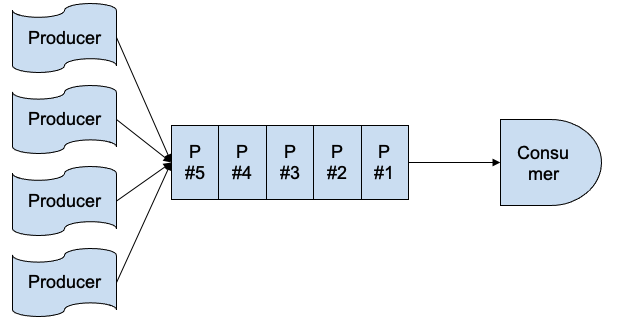
\includegraphics[width=\linewidth]{images/h9/opgave_producer_consumer.png}
\caption{Producers en consumer}
\label{fig:producer_consumer}
\end{figure}

\textbf{Package}\\
De Package klasse is reeds gegeven, deze bevat enkel een constructor die een ID of volgnummer toekent aan elk nieuw pakketje op de lijn en voorziet ook een toString methode. Hiervoor wordt een klasse variabele gebruikt, deze waarde moet dus niet meegegeven worden bij de creatie van een Package.
\\
\textbf{ProductionLine}\\
Maak een ProductionLine klasse die de productielijn zal voorstellen. Op de productielijn kan je nieuwe producten enkel achteraan toevoegen en enkel vooraan afnemen. Gebruik een verzameling naar keuze uit het Collection framework. Voorzie methoden om een Package toe te voegen aan het einde van de productielijn ( addPackage() ) en om een Package aan de voorkant af te nemen. ( getPackage() ) Denk eraan om de afgenomen pakketjes ook van de productielijn te verwijderen. 
Zorg dat er geen exceptions kunnen optreden als er geen pakketjes meer op de lijn zitten.
Voorzie het nodige om ervoor te zorgen dat alle bewerkingen op de productielijn gesynchroniseerd verlopen en dat het dus niet mogelijk is dat meerdere threads tegelijk een bewerking op de verzameling uitvoeren. (Hiervoor moet je enkel aanpassingen doen op de methoden addPackage() en getPackage() van de ProductionLine klasse.
\\
\textbf{Producer}\\
Maak de Producer klasse aan. Deze zal aan een vast tempo nieuwe Packages aanmaken en deze aan de productielijn toevoegen. De Producer moet kunnen runnen als een thread, dus voorzie daar het nodige voor. In de constructor moet je twee parameters voorzien: de rate waaraan nieuwe producten aangemaakt worden en het productielijn object. De rate is het aantal pakketjes dat deze consumer per minuut aanmaakt.
Wanneer de Producer thread opgestart wordt, moet deze continu nieuwe Packages aanmaken en aan de productielijn toevoegen, met tussenin telkens een pauze zodat de aangegeven rate aangehouden wordt (gebruik hiervoor Thread.sleep(milliseconds)). De thread geeft een korte melding in de console weer, telkens wanneer er een nieuw pakketje op de lijn geplaatst wordt.
Het juiste aantal milliseconden dat de Producer moet wachten tussen 2 pakketjes kan je als volgt berekenen: (60 / rate) * 1000
\\
\textbf{Consumer}\\
De Consumer klasse is gelijkaardig: deze moet ook kunnen runnen als een thread en in de constructor worden eveneens de rate (= opnieuw het aantal pakketjes dat de Consumer per minuut kan verwerken) en het productielijn object meegegeven.
Na opstarten zal de Consumer continu pakketjes van de productielijn afnemen (telkens vooraan) aan de opgegeven rate. Gebruik de methode die je hiervoor voorzien hebt in de ProductionLine klasse. 
De thread print telkens uit welk pakket verwerkt werd. Ook wanneer er geen pakketjes beschikbaar zijn op de productielijn, wordt dit gemeld via een bericht in de console.
\\
\textbf{Main methode}\\
Voorzie tenslotte een main methode. Deze gebruik je om 4 Producers aan te maken met de rates 20, 15, 12 en 7. Daarna maak je ook een Consumer aan met als rate 30. De Consumer verwerkt dus 30 pakketjes per minuut en werkt daarmee sneller dan de 4 Producers. 
Zorg dat al deze componenten correct opgestart worden en parallel hun werk doen. Op deze manier zou je moeten kunnen analyseren of de Consumer voldoende snel werkt om de 4 gelijktijdige Producers aan te kunnen.
\end{oefening}


4. Synchronization and Locks
Synchronized Methods and Blocks
Object and Class Level Locks
Deadlocks, Livelocks, and How to Avoid Them
Lock Objects in java.util.concurrent.locks
5. Advanced Thread Coordination
Wait/Notify Mechanisms
Using Conditions and ReentrantLock
CountDownLatch, CyclicBarrier, and Semaphore
6. Concurrency Utilities (java.util.concurrent)
Executors and Thread Pools
Fixed thread pool
Cached thread pool
Scheduled thread pool
Work-stealing pool
Concurrent Collections (e.g., ConcurrentHashMap, BlockingQueue)
Atomic Variables and java.util.concurrent.atomic package
8. Parallel Streams
Creating Parallel Streams
Performance Considerations
Use Cases for Parallel vs. Sequential Streams
9. Asynchronous Programming
Using CompletableFuture
Combining CompletableFutures
Exception Handling in Asynchronous Code
Link to Spring Asynchronous Methods Guide
